\section{User Interface Design}
    % Questo comando assicura che tutti i bottoni abbiano lo stesso stile (Grassetto + Corsivo)
    \newcommand{\uiElement}[1]{\textit{\textbf{#1}}}
    % ---------------------------------------------------------------------

    \subsection{Overview}
    The BBP user interface is designed according to "Minimal Attention UX" principles to ensure safety during mobile use.
    While the RASD defined the visual appearance through mockups, this section details the navigation logic and the structure of the transitions 
    between views, organized by functional areas.
    \pagebreak
    
    \subsection{Navigation Logic}

    \subsubsection{Entry Point and Authentication Flow}
    Access to the system is managed through the \textit{Login} screen, which acts as the main hub to direct the user towards the authenticated or 
    anonymous flow.

    \begin{figure}[H]
        \centering
        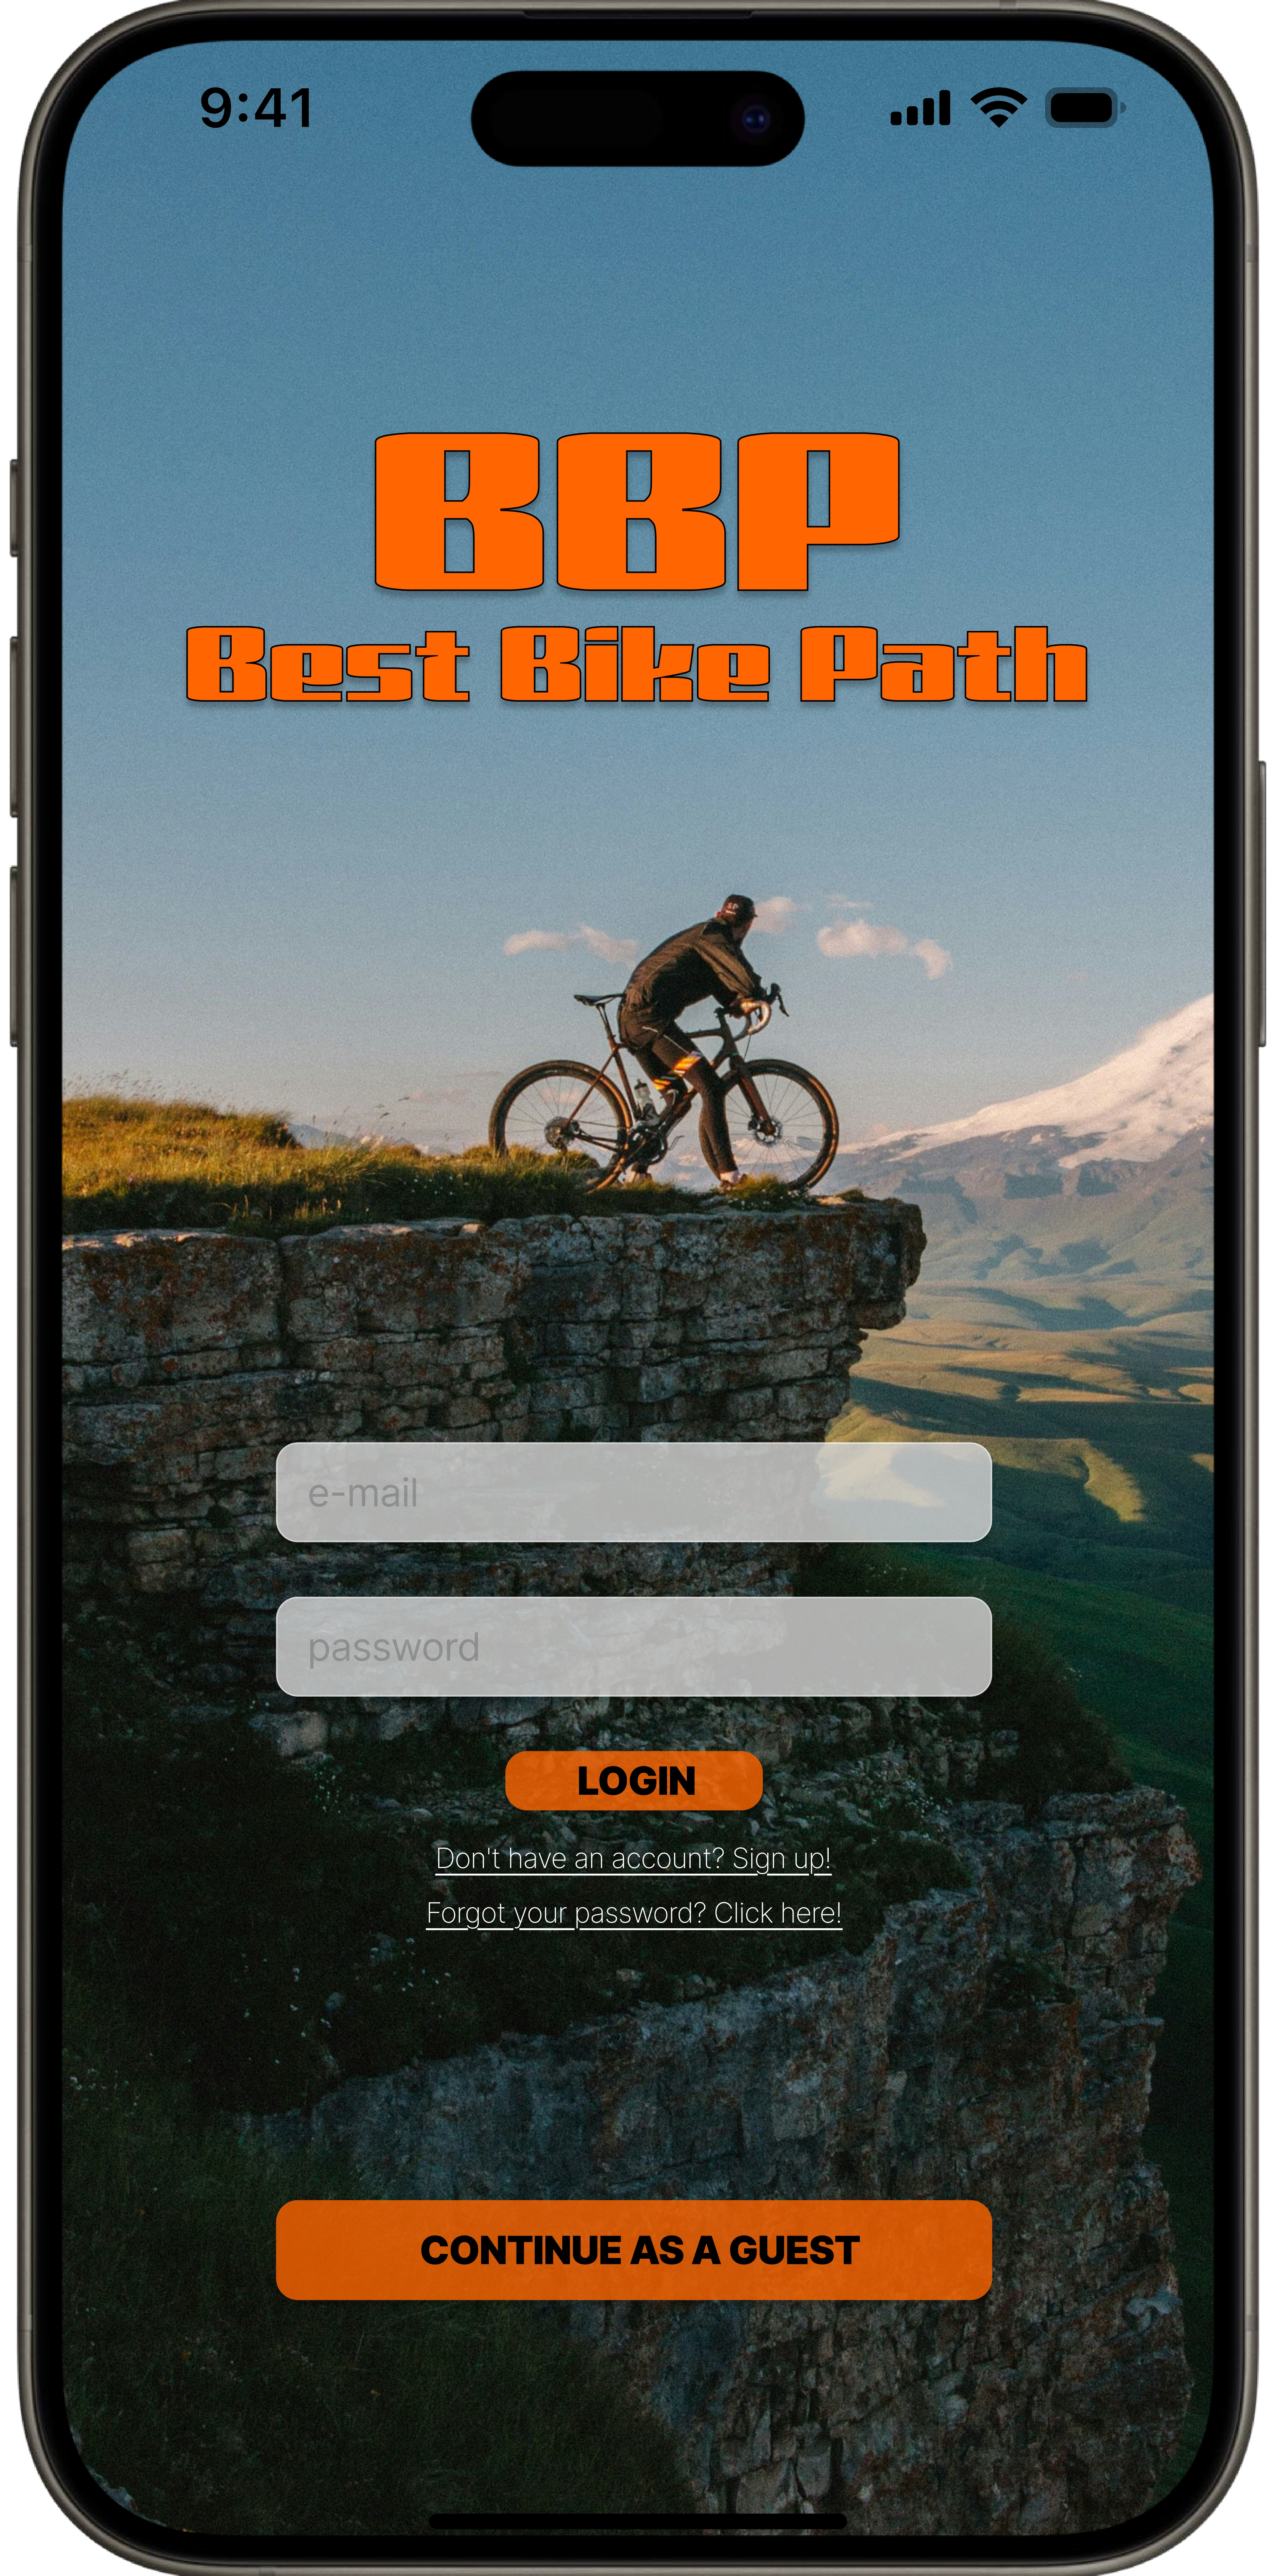
\includegraphics[width=0.5\textwidth]{RASD/mockups/mockup_login.jpg} 
        \caption{Start Screen and Access Logic}
        \label{fig:ui_login}
    \end{figure}

    \textbf{Transitions and Logic:}
    \begin{itemize}
        \item \textbf{Guest Path:} The \uiElement{Continue As A Guest} button instantiates an anonymous session and redirects the user directly to the 
        \textit{Map View} (see Fig. \ref{fig:ui_map}) with limited functionality.
        
        \item \textbf{Registered Path:} Entering credentials and tapping \uiElement{Login} validates the token; if successful, the user is redirected to the 
        \textit{Map View} with the Bottom Bar enabled.
        
        \item \textbf{Registration:} The \uiElement{Sign up} link opens the registration form, which, once completed, returns to this screen for the first login.
        
        \item \textbf{Password Recovery:} The \uiElement{Forgot your password?} link starts the external credential recovery flow via secure email. Once the 
        process is complete, the user remains on this screen to log in with the new password.
    \end{itemize}
    \pagebreak

    \subsubsection{Core Experience: Search and Tracking}
    The map is the central view of the application. From here, the user plans and takes action.

    \begin{figure}[H]
        \centering
        \includegraphics[width=0.5\textwidth]{RASD/mockups/mockup_search.jpg}
        \caption{Main Map View and Route Selection}
        \label{fig:ui_map}
    \end{figure}

    \textbf{Transitions and Logic:}
    \begin{itemize}
        \item \textbf{Route Selection:} Interacting with search results or tracks on the map updates the Bottom Sheet shown in the figure.
        
        \item \textbf{Start Navigation:} The \uiElement{Start} button initializes the Tracking state, placing the interface in "Driving Mode".
        
        \item \textbf{Alerts:} The \uiElement{List Alert} button opens a modal overlay listing known obstacles on the route.
        
        \item \textbf{Automatic Mode:} The \uiElement{Automatic mode} toggle switch allows the user to explicitly enable or disable sensor data acquisition for 
        the upcoming trip.
        
        \item \textbf{Sharing:} The \uiElement{Share} icon (top right) activates the operating system's native share sheet for sharing the route with other users.
        
        \item \textbf{Text View:} The \uiElement{List} icon (top left of the panel) switches the view from the graphical map to a text list of navigation directions.
    \end{itemize}
    \pagebreak
    
    \subsubsection{Data Governance Flow}
    At the end of a tracking session, the system prevents an immediate return to the Home page, forcing a critical data validation step.

    \begin{figure}[H]
        \centering
        \includegraphics[width=0.5\textwidth]{RASD/mockups/mockup_confirmation.jpg}
        \caption{Confirmation and Data Validation Screen}
        \label{fig:ui_confirm}
    \end{figure}

    \textbf{Transitions and Logic:}
    \begin{itemize}
        \item \textbf{Loop Closure:} This view is accessible only after the \texttt{Stop Recording} event and represents the mandatory Data Governance step.
        
        \item \textbf{Immediate Feedback:} The \uiElement{Trip Statistics} section immediately displays a summary of the performance metrics calculated
        for the trip just completed, such as distance, duration, average speed, etc.
        
        \item \textbf{Automatic Validation:} The \uiElement{Confirm} / \uiElement{Decline} toggles allow the user to validate or reject anomalies detected by the sensors, 
        preventing false positives.
        
        \item \textbf{Manual Enrichment:} The \uiElement{Do you want to add anything else?} button opens a context menu that allows the user to manually 
        report any issues not detected by the sensors or add specific details.
        
        \item \textbf{Qualitative Evaluation:} The \uiElement{Path Status} selector allows the user to assign an overall rating on the condition of the path 
        just completed (e.g., Optimal, Average, Poor).
        
        \item \textbf{Exit and Persistence:} The \uiElement{End Trip} button is the only way out: it finalizes the session, saves the confirmed data to the remote 
        database, and redirects the user to the \textit{History/Profile} view (Fig. \ref{fig:ui_history}).
    \end{itemize}
    \pagebreak

    \subsubsection{Persistence and History}
    The personal area allows asynchronous consultation of saved data.

    \begin{figure}[H]
        \centering
        \includegraphics[width=0.5\textwidth]{RASD/mockups/mockup_history.jpg}
        \caption{View Trip History}
        \label{fig:ui_history}
    \end{figure}

    \textbf{Transitions and Logic:}
    \begin{itemize}
        \item \textbf{Access:} Accessible via the \uiElement{Profile} tab in the Bottom Navigation Bar.
        \item \textbf{Detail:} Tapping on a card in the list opens the detail view of the individual trip.
    \end{itemize}